\documentclass[a4paper]{article}

\usepackage[margin=2cm]{geometry}
\usepackage[utf8]{inputenc}
\usepackage{booktabs}
\usepackage[fleqn]{amsmath}
\usepackage{amsfonts}
\usepackage{amssymb}
\usepackage{float}
\usepackage{tikz}
\usepackage{color}
\usepackage{caption}
\usepackage{listings}
\usepackage{graphicx}
\usepackage{struktex}

\definecolor{mygreen}{rgb}{0,0.6,0}
\definecolor{mygray}{rgb}{0.5,0.5,0.5}
\definecolor{mymauve}{rgb}{0.58,0,0.82}
\definecolor{light-gray}{gray}{0.95}

\lstset
{
    language=C++,
    backgroundcolor=\color{light-gray},
    basicstyle=\ttfamily\linespread{1.15}\footnotesize,
    numbers=left,
    stepnumber=1,
    showstringspaces=false,
    tabsize=1,
    breaklines=true,
    breakatwhitespace=false,
    commentstyle=\color{mygreen},
    keywordstyle=\color{blue},
    stringstyle=\color{mymauve},
}

\usetikzlibrary{shapes.geometric, arrows}
\tikzstyle{box} = [rectangle, minimum width=3cm, minimum height=1cm, text centered, draw=black]
\tikzstyle{arrow} = [thin, -, >=stealth]

\graphicspath{{./IMG/}}

\title{”Programozás”\\ beadandó feladat:\\ 4. feladat}
\date{2017-03-06}
\author{Készítette: Bárdosi Bence\\ Neptun-azonosító: VY9NJN\\ E-mail: bardosi.bence@gmail.com}

\renewcommand*\contentsname{Tartalom}
\renewcommand*\figurename{}


\begin{document}
  \pagenumbering{gobble}
  \maketitle
  \newpage

  \pagenumbering{arabic}
  \tableofcontents
  \newpage

  \section{Dokumentáció}
    \subsection{Feladat}
    Madarak életének kutatásával foglalkozó szakemberek n különböző településen m különböző madárfaj előfordulását tanulmányozzák. Egy adott időszakban megszámolták, hogy az egyes településen egy madárfajnak hány egyedével találkoztak.
    Volt-e olyan település, ahol mindegyik madárfaj előfordult?
    \subsection{Specifikáció}
    \begin{align*}
      \mathbf{A=}\, \left ( adat: \mathbb{N}^{n x m} , l: \mathbb{L} \right )
    \end{align*}
    \begin{align*}
      \mathbf{Ef=}\, \left ( adat=adat' \right )
    \end{align*}
    \begin{align*}
      \mathbf{Uf=}\, \left ( Ef \wedge (l,\_)=\sum_{i=1}^n mind(adat[i]) \right )
    \end{align*}
    \begin{align*}
      \mathbf{ahol\, mind(adat[i]):}
    \end{align*}
    \begin{align*}
      \mathbf{A=}\, \left ( sor: adat[i] (\mathbb{N}^{m}) , l: \mathbb{L} \right )
    \end{align*}
    \begin{align*}
      \mathbf{Ef=}\, \left ( sor=sor' \right )
    \end{align*}
    \begin{align*}
      \mathbf{Uf=}\, \left ( Ef \wedge l=\forall \sum_{i=1}^m sor[i]>0 \right )
    \end{align*}
    \subsection{Algoritmus}
      A feladatot a lineáris keresés, az alfeladatot az optimista lineáris keresés programozási tételeire vezetjük vissza.
      \begin{table}[H]
        \caption*{Lineáris keresés}
        \begin{tabular*}{0.55\textwidth}{ccc}
          \toprule
          Tétel & & Feladat \\
          \midrule
          $m$ & $\leftarrow$ & 1 \\
          $n$ & $\leftarrow$ & n \\
          $ind$ & $\leftarrow$ & $\_$ \\
          $\beta (i)$ & $\leftarrow$ & $\sum_{i=1}^n mind(adat[i])$ \\
          \bottomrule
        \end{tabular*}
      \end{table}
      \begin{table}[H]
        \caption*{Optimista lineáris keresés}
        \begin{tabular*}{0.55\textwidth}{ccc}
          \toprule
          Tétel & & Feladat \\
          \midrule
          $m$ & $\leftarrow$ & 1 \\
          $n$ & $\leftarrow$ & m \\
          $\beta (i)$ & $\leftarrow$ & $\forall \sum_{i=1}^m sor[i]>0$ \\
          \bottomrule
        \end{tabular*}
      \end{table}
      \begin{struktogramm}(100,25)
  \assign{\(c:=0\)}
  \while{\(i:=2..n\)}
   \ifthenelse{6}{6}{\(T[i]<0 \acute es\ T[i-1]=0\)}{i}{n}
    \assign{\(c:=c+1\)}
   \change
   \ifend
  \whileend
\end{struktogramm}

    \subsection{Implementáció}
        \subsubsection{Adattípusok megvalósítása}
        A kódoláskor a t tömböt \texttt{vector<float>}-ként deklaráljuk, amelynek mérete \texttt{t.size()} alakban érhető el. Mivel a vektor 0-tól indexelődik, azért a tervbeli ciklus nem a \texttt{2..n}, hanem az 1..n-1 intervallumot, pontosabban a \texttt{1..t.size()-1} intervallumot futja be, aminek következtében a struktogramm kódja az alábbi lesz:
        \begin{lstlisting}
        int c=0;
        for(int i=1; i<(int)t.size(); ++i)
            if(t[i]<0 && t[i-1]==0)
                ++c;}
        \end{lstlisting}
        \subsubsection{Bemenő adatok formája}
        A bemenő adatokat egy szöveges állományból kell a tömbbe bemásolni. Az állományban a megadott értékeket szóközökkel, tabulátor jelekkel vagy sorvége jelekkel elválasztva kell beírni. Az állomány minden sorát sorvége jel zárja le.
      \subsubsection{Függvények kapcsolódási szerkezete}
        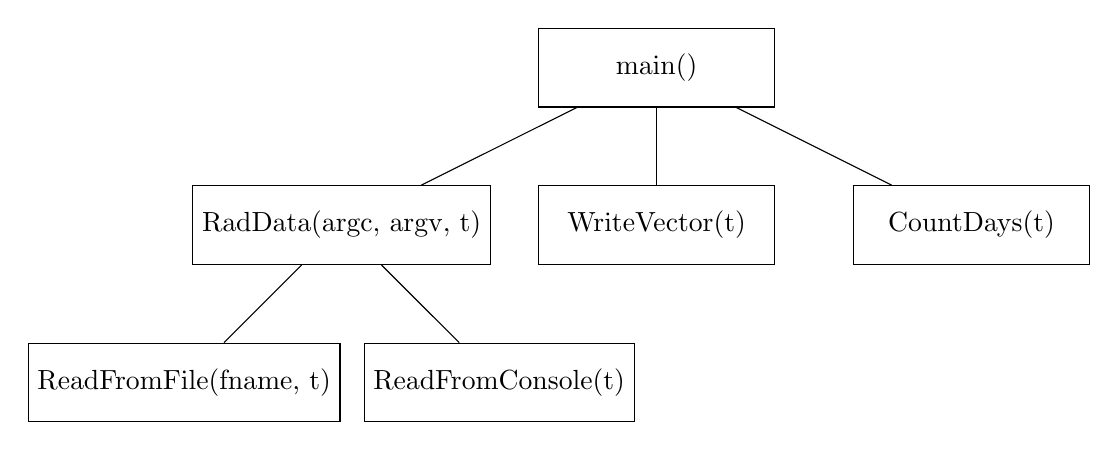
\begin{tikzpicture}[node distance=2cm]
          \node (write) [box] {WriteVector(t)};
          \node (fo) [box, above of=write] {main()};
          \node (beolv) [box, left of=write, xshift=-2cm] {RadData(argc, argv, t)};
          \node (cnt) [box, right of=write, xshift=2cm] {CountDays(t)};
          \node (file) [box, below of=beolv, xshift=-2cm] {ReadFromFile(fname, t)};
          \node (cons) [box, right of=file, xshift=2cm] {ReadFromConsole(t)};
          \draw [arrow] (fo) -- (write);
          \draw [arrow] (fo) -- (beolv);
          \draw [arrow] (fo) -- (cnt);
          \draw [arrow] (beolv) -- (file);
          \draw [arrow] (beolv) -- (cons);
        \end{tikzpicture}
    \subsection{Tesztelés}
      \subsubsection{A feladat specifikációjára épülő (fekete doboz) tesztesetek:}
      \begin{table}[H]
        \caption*{}
        \begin{tabular*}{\textwidth}{ll}
          \toprule
          \textbf{Megszámlálás tétel} tesztesetei: & \\
          \textbf{intervallum hossza} szerint: & \\
          1. \textit{nulla} hosszú: & Egyetlen nap sincs \\
          & \quad be1.txt: [] - válasz: 0 \\
          2. \textit{egy} hosszú: & Egyetlen nap \\
          & \quad be2.txt: [5.2] - válasz: 0 \\
          3. \textit{kettő} hosszú: & Kettő, a feltételnek eleget nem tevő nap \\
          & \quad be3.txt: [5.2, 0] - válasz: 0 \\
          & Kettő, a feltételnek eleget tevő nap \\
          & \quad be3.txt: [0, -2] - válasz: 1 \\
          4. \textit{több} hosszú: & Több nap \\
          & \quad be5.txt: [0, -2, 0, 5, 6, 0, -0.5] - válasz: 2 \\
          \textbf{intervallum eleje} szerint: & \\
          & Sorozat elején található csak a feltételnek megfelelő nappár \\
          & \quad be6.txt: [0, -2, 0, 5, 6, 0] - válasz: 1 \\
          \textbf{intervallum vége} szerint: & \\
          & Sorozat végén található csak a feltételnek megfelelő nappár \\
          & \quad be7.txt: [0, 2, 0, 5, 6, 0, -2] - válasz: 1 \\
          \textbf{tételre jellemző esetek} szerint: & \\
          1. Egyetlen megfelelő nappár van: & \\
          & \quad be7.txt: [0, 2, 0, 5, 6, 0, -2] - válasz: 1 \\
          2. Nincs megfelelő nappár: & \\
          & \quad be8.txt: [0, 1, 2, 3, 4] - válasz: 0 \\
          3. Egy "0" napot több "negatív" nap követ: & \\
          & \quad be9.txt: [1, 2, 0, -1, -2, -1] - válasz: 0 \\
          \bottomrule
        \end{tabular*}
      \end{table}
    \subsubsection{A megoldó programra épülő (fehér doboz) tesztesetek:}
      \begin{itemize}
        \item Hibás vagy nem létező állománynév megadása.
        \item Állomány nevének megadása parancssorból.
        \item Olyan állomány olvasása, ahol egy sorban több érték is található egyetlen illetve több szóközzel és/vagy tabulátor jellel elválasztva (be10.txt).
        \item Olyan állomány olvasása, ahol minden érték külön sorban van (be9.txt).
        \item Olyan állomány olvasása, ahol az utolsó sort nem zárja sorvége jel, és éppen ennek a sornak a tartalma határozza meg az eredményt (adat: [1, 2, 3, 0, -1] – válasz: 1) (be11.txt).
        \item Főprogram ciklusának ellenőrzése: olyan bemenő adatokkal, amelyekre a ciklus egyszer sem fut le (Pl: be1.txt), pontosan egyszer fut le (Pl: be3.txt), vagy többször lefut(Pl:be5.txt).
      \end{itemize}


\end{document}
